% Figure 1 -- architecture of the study. Compile with pdflatex; the result is
% copied to ../figures/Figure_1.pdf (vector, fonts embedded) by build_submission.py.
\documentclass[border=2pt]{standalone}
\usepackage{times}
\usepackage[T1]{fontenc}
\usepackage{amsmath}
\usepackage{tikz}
\usetikzlibrary{arrows.meta,positioning,calc,fit,backgrounds}
\hyphenpenalty=10000 \exhyphenpenalty=10000

% Colour-blind-safe tints; outlines and text keep the figure legible in grey.
\definecolor{sA}{RGB}{222,235,247}   % corpus
\definecolor{sB}{RGB}{226,240,217}   % pool and measurement
\definecolor{sC}{RGB}{255,242,204}   % labels and routers
\definecolor{sD}{RGB}{237,226,246}   % policies and accounting
\definecolor{sE}{RGB}{236,236,236}   % wider pools
\definecolor{edge}{RGB}{50,50,50}

\tikzset{
  box/.style={draw=edge, fill=white, line width=0.5pt, rounded corners=1.5pt,
              align=flush left, inner sep=3pt, font=\fontsize{7.2}{8.6}\selectfont},
  head/.style={font=\fontsize{8}{9.5}\selectfont\bfseries, align=center},
  flow/.style={-{Stealth[length=4pt,width=3.2pt]}, line width=0.6pt, color=edge},
  wire/.style={line width=0.6pt, color=edge},
  tag/.style={font=\fontsize{6.6}{7.8}\selectfont\itshape, color=edge, inner sep=1.5pt},
  c1/.style={box, text width=3.2cm},
  c2/.style={box, text width=3.55cm},
  c3/.style={box, text width=3.55cm},
  c4/.style={box, text width=3.35cm},
  gap/.style={node distance=0.42cm},
}

\begin{document}
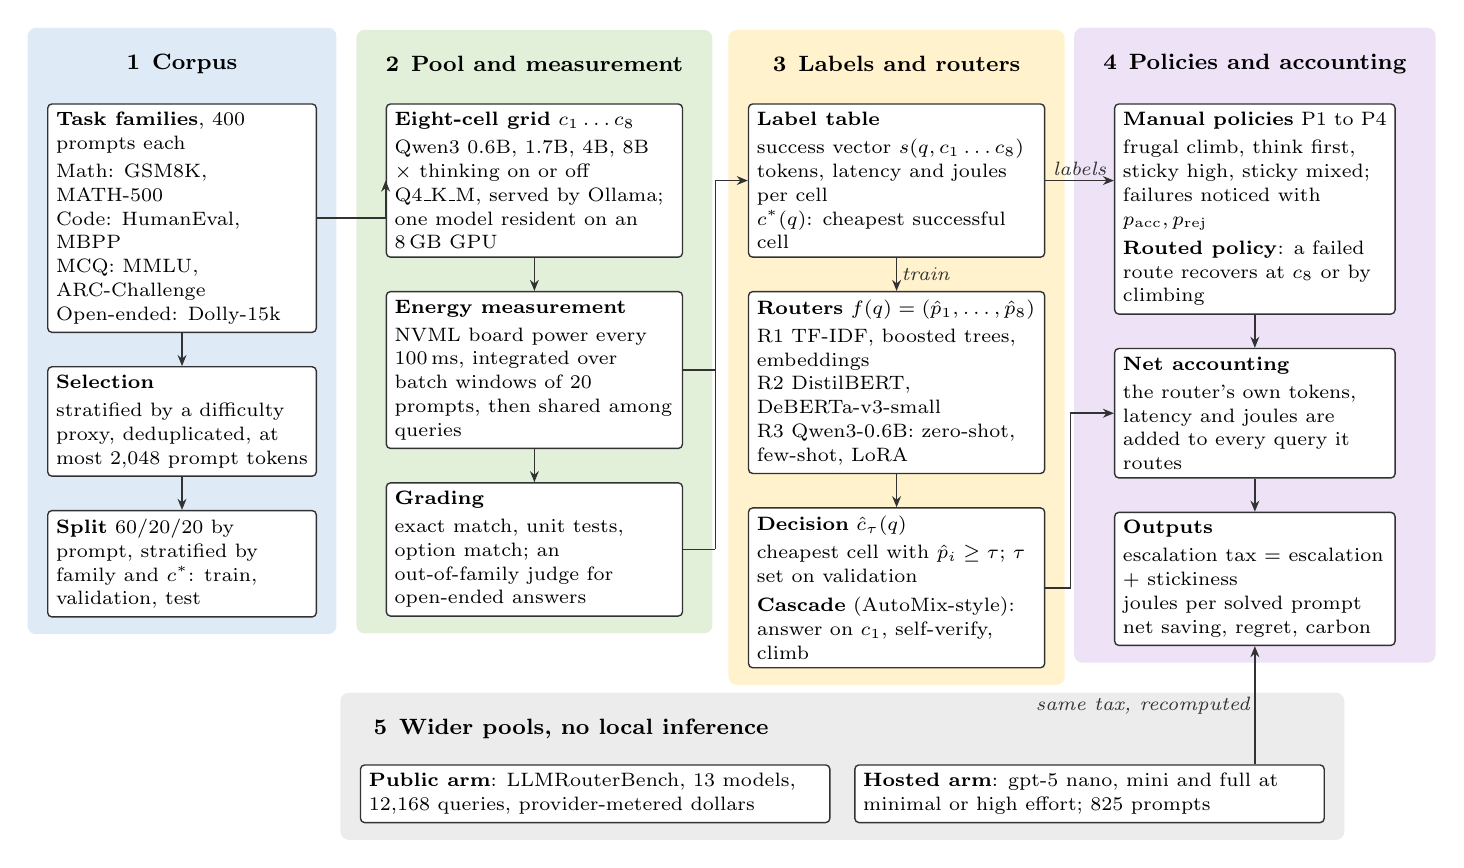
\begin{tikzpicture}[x=1cm,y=1cm]

% ------------------------------------------------------------------ 1 corpus
\node[c1, anchor=north west] (fam) at (0.2,0)
  {\textbf{Task families}, 400 prompts each\\[1.5pt]
   Math: GSM8K, MATH-500\\
   Code: HumanEval, MBPP\\
   MCQ: MMLU, ARC-Challenge\\
   Open-ended: Dolly-15k};
\node[c1, gap, below=of fam] (sel)
  {\textbf{Selection}\\[1.5pt]
   stratified by a difficulty proxy, deduplicated, at most 2,048 prompt tokens};
\node[c1, gap, below=of sel] (spl)
  {\textbf{Split} 60/20/20 by prompt, stratified by family and $c^{*}$: train, validation, test};
\draw[flow] (fam) -- (sel);
\draw[flow] (sel) -- (spl);

% ------------------------------------------------------- 2 pool and measurement
\node[c2, anchor=north west] (grid) at (4.5,0)
  {\textbf{Eight-cell grid} $c_1\dots c_8$\\[1.5pt]
   Qwen3 0.6B, 1.7B, 4B, 8B\\
   $\times$ thinking on or off\\
   Q4\_K\_M, served by Ollama; one model resident on an 8\,GB GPU};
\node[c2, gap, below=of grid] (nvml)
  {\textbf{Energy measurement}\\[1.5pt]
   NVML board power every 100\,ms, integrated over batch windows of 20 prompts, then shared among queries};
\node[c2, gap, below=of nvml] (grade)
  {\textbf{Grading}\\[1.5pt]
   exact match, unit tests, option match; an out-of-family judge for open-ended answers};
\draw[flow] (grid) -- (nvml);
\draw[flow] (nvml) -- (grade);

% ----------------------------------------------------------- 3 labels, routers
\node[c3, anchor=north west] (lab) at (9.1,0)
  {\textbf{Label table}\\[1.5pt]
   success vector $s(q,c_1\dots c_8)$\\
   tokens, latency and joules per cell\\
   $c^{*}(q)$: cheapest successful cell};
\node[c3, gap, below=of lab] (rout)
  {\textbf{Routers} $f(q)=(\hat p_1,\dots,\hat p_8)$\\[1.5pt]
   R1 TF-IDF, boosted trees, embeddings\\
   R2 DistilBERT, DeBERTa-v3-small\\
   R3 Qwen3-0.6B: zero-shot, few-shot, LoRA};
\node[c3, gap, below=of rout] (tau)
  {\textbf{Decision} $\hat c_\tau(q)$\\[1.5pt]
   cheapest cell with $\hat p_i\ge\tau$; $\tau$ set on validation\\[2pt]
   \textbf{Cascade} (AutoMix-style): answer on $c_1$, self-verify, climb};
\draw[flow] (lab) -- node[right,tag]{train} (rout);
\draw[flow] (rout) -- (tau);

% ------------------------------------------------- 4 policies and accounting
\node[c4, anchor=north west] (pol) at (13.75,0)
  {\textbf{Manual policies} P1 to P4\\[1.5pt]
   frugal climb, think first, sticky high, sticky mixed; failures noticed with $p_{\mathrm{acc}},p_{\mathrm{rej}}$\\[2pt]
   \textbf{Routed policy}: a failed route recovers at $c_8$ or by climbing};
\node[c4, gap, below=of pol] (net)
  {\textbf{Net accounting}\\[1.5pt]
   the router's own tokens, latency and joules are added to every query it routes};
\node[c4, gap, below=of net] (out)
  {\textbf{Outputs}\\[1.5pt]
   escalation tax $=$ escalation $+$ stickiness\\
   joules per solved prompt\\
   net saving, regret, carbon};
\draw[flow] (pol) -- (net);
\draw[flow] (net) -- (out);

% ---------------------------------------------------------- stage panels
\node[head] (h1) at ($(fam.north)+(0,0.5)$) {1\;\,Corpus};
\node[head] (h2) at ($(grid.north)+(0,0.5)$) {2\;\,Pool and measurement};
\node[head] (h3) at ($(lab.north)+(0,0.5)$) {3\;\,Labels and routers};
\node[head] (h4) at ($(pol.north)+(0,0.5)$) {4\;\,Policies and accounting};
\begin{pgfonlayer}{background}
  \node[fill=sA, rounded corners=3pt, inner xsep=7pt, inner ysep=6pt, fit=(h1)(fam)(sel)(spl)] (p1) {};
  \node[fill=sB, rounded corners=3pt, inner xsep=7pt, inner ysep=6pt, fit=(h2)(grid)(nvml)(grade)] (p2) {};
  \node[fill=sC, rounded corners=3pt, inner xsep=7pt, inner ysep=6pt, fit=(h3)(lab)(rout)(tau)] (p3) {};
  \node[fill=sD, rounded corners=3pt, inner xsep=7pt, inner ysep=6pt, fit=(h4)(pol)(net)(out)] (p4) {};
\end{pgfonlayer}

% --------------------------------------------------------- 5 wider pools
\node[head, anchor=west] (h5) at ($(p2.south west |- p3.south)+(0.1,-0.55)$)
  {5\;\,Wider pools, no local inference};
\node[box, text width=5.75cm, anchor=north west] (pub) at ($(h5.south west)+(-0.05,-0.2)$)
  {\textbf{Public arm}: LLMRouterBench, 13 models, 12,168 queries, provider-metered dollars};
\node[box, text width=5.75cm, anchor=north west] (hos) at ($(pub.north east)+(0.3,0)$)
  {\textbf{Hosted arm}: gpt-5 nano, mini and full at minimal or high effort; 825 prompts};
\begin{pgfonlayer}{background}
  \node[fill=sE, rounded corners=3pt, inner xsep=7pt, inner ysep=6pt, fit=(h5)(pub)(hos)] (p5) {};
\end{pgfonlayer}

% ------------------------------------------------------------------ data flow
% prompts -> grid
\draw[flow] (fam.east) -- (grid.west |- fam.east) -- (grid.west);
% grading and energy both feed the label table
\coordinate (bus) at ($(grade.east)!0.5!(lab.west)$);
\draw[wire] (grade.east) -- (grade.east -| bus);
\draw[wire] (nvml.east) -- (nvml.east -| bus);
\draw[wire] (grade.east -| bus) -- (lab.west -| bus);
\draw[flow] (lab.west -| bus) -- (lab.west);
% labels -> policies; the decision and the router's cost -> accounting
\draw[flow] (lab.east) -- node[above,tag]{labels} (pol.west |- lab.east);
\draw[flow] (tau.east) -- ++(0.32,0) |- (net.west);
% wider pools reuse the policy code and report the same tax
\draw[flow] (hos.north -| out.south) -- node[left,tag]{same tax, recomputed} (out.south);

\end{tikzpicture}
\end{document}
